\PassOptionsToPackage{table}{xcolor}
\documentclass[aspectratio=169]{beamer}\usepackage[utf8]{inputenc}
\usepackage{lmodern}
\usepackage[english]{babel}
\usepackage{color}
\usepackage{amsmath,mathtools}
\usepackage{booktabs}
\usepackage{mathptmx}
\usepackage[11pt]{moresize}
\usepackage{hyperref}
\usepackage{commath}
\usepackage{bm}
\usepackage{subfigure}
\usepackage{siunitx}

\setbeamertemplate{navigation symbols}{}
\setbeamersize{text margin left=5mm,text margin right=5mm}
\setbeamertemplate{caption}[numbered]
\addtobeamertemplate{navigation symbols}{}{
\usebeamerfont{footline}
\usebeamercolor[fg]{footline}
\hspace{1em}
\insertframenumber/\inserttotalframenumber}

\newcommand{\R}{\mathbb{R}}
\newcommand{\E}{\mathbb{E}}
\newcommand{\N}{\mathbb{N}}
\newcommand{\Z}{\mathbb{Z}}
\newcommand{\V}{\mathbb{V}}
\newcommand{\Q}{\mathbb{Q}}
\newcommand{\K}{\mathbb{K}}
\newcommand{\C}{\mathbb{C}}
\newcommand{\T}{\mathbb{T}}
\newcommand{\I}{\mathbb{I}}

\title{Advances Report}
\subtitle{Renzo Miguel Caballero Rosas}

\begin{document}

\begin{frame}
\titlepage
\end{frame}

\setbeamercolor{background canvas}{bg=white!10}
\begin{frame}\frametitle{Introduction}

The main idea is to achieve a self-repairing 3D printer. When a part is broken/damaged, the 3D printer will either print or order a replacement online.\\
\quad\\
The starting point is to assume a damaged timing pulley and check if we can print a new one while the printer has the damaged one. Even when the first printing may not be perfect, it may be better than the damaged one, and then we can replace it and try again until we converge to a suitable part.

\end{frame}


\setbeamercolor{background canvas}{bg=white!10}
\begin{frame}\frametitle{Damaged pulley}



\begin{columns}[c]

\column{.45\textwidth}
To simulate a damaged pulley we use a triangular one. We use this shape since it is way different from a circular one.\\
\quad\\
We choose an edge's length for the triangle that guarantees no modification in the belt's tension with respect to the original pulley.

\column{.45\textwidth}
\begin{figure}[ht!]
\centering
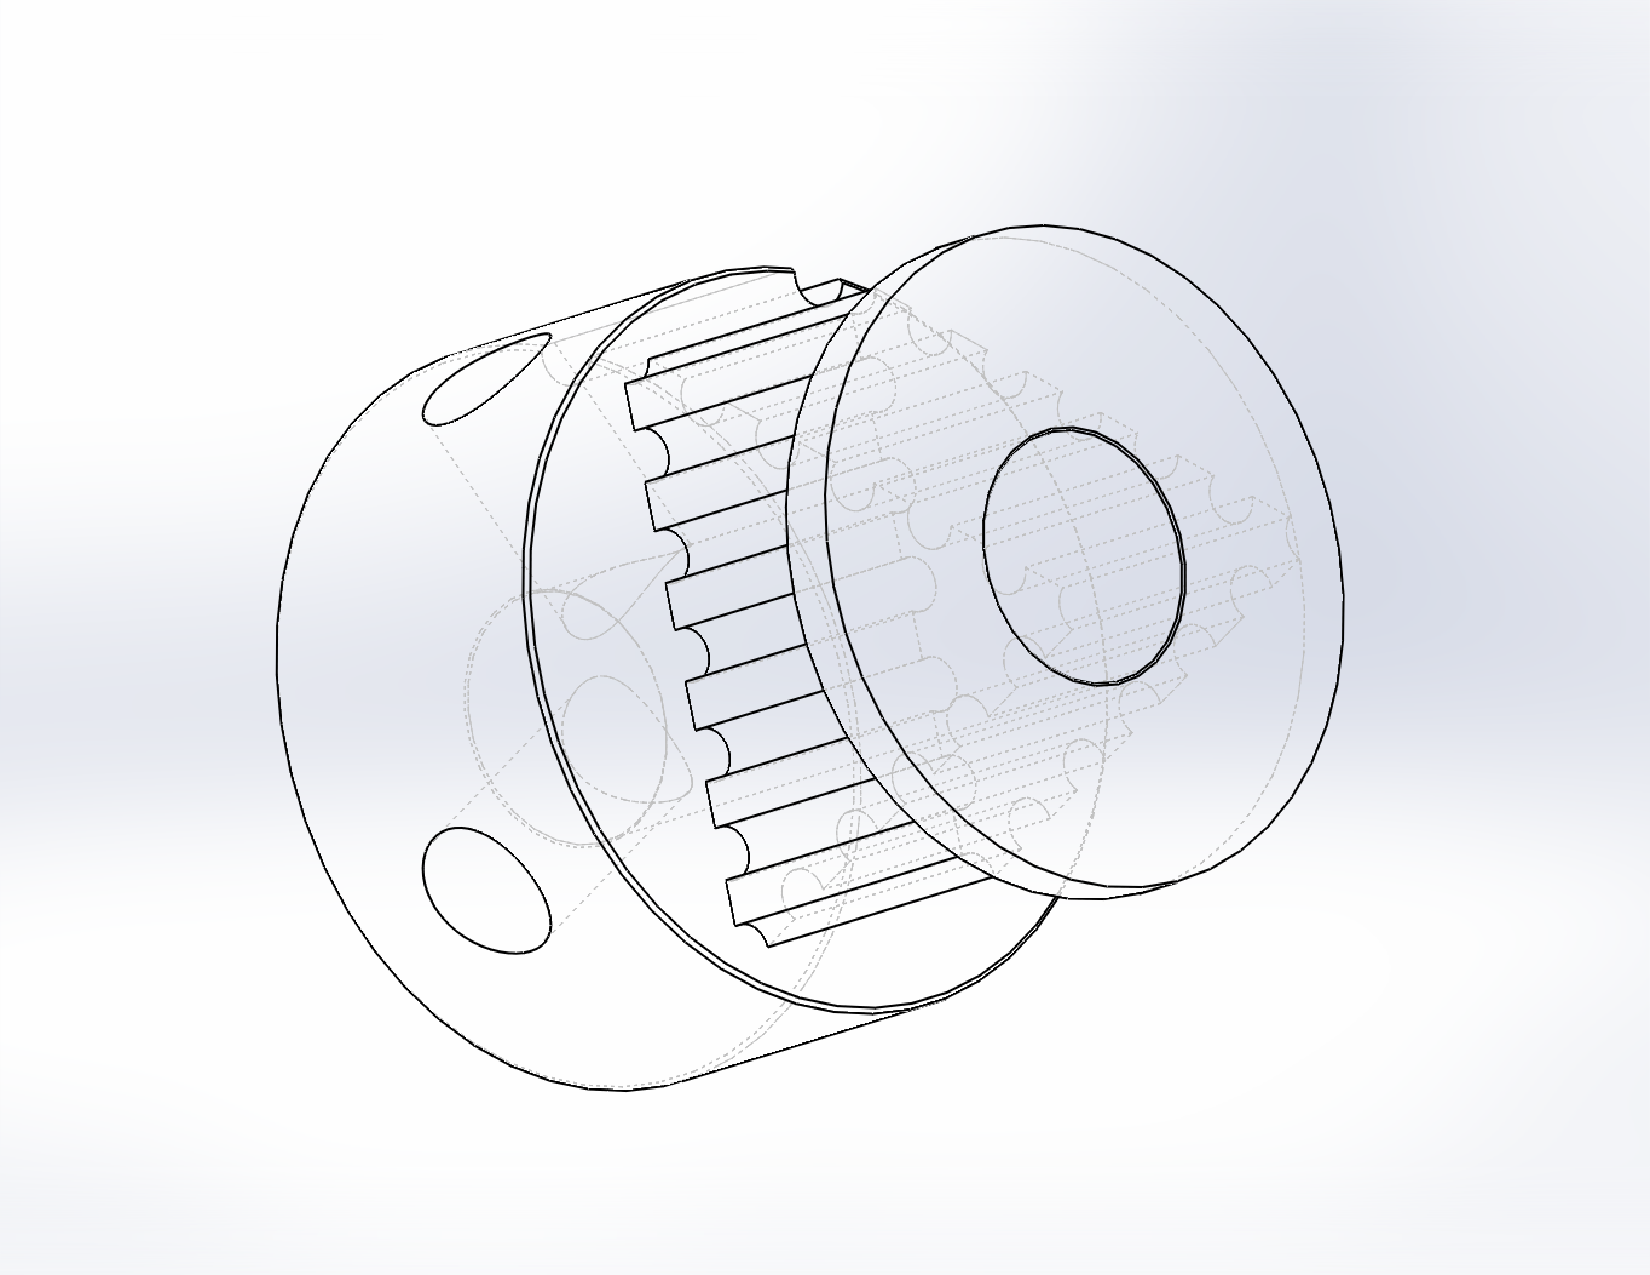
\includegraphics[width=1\textwidth]{figures/pulley_tri_small.PDF}
\end{figure}

\end{columns}

\end{frame}



\setbeamercolor{background canvas}{bg=white!10}
\begin{frame}\frametitle{Iterations}

\begin{figure}[ht!]
\centering
\includegraphics[width=1\textwidth]{Figures/pic_ite.png}
\caption{On the left: Initial triangular pulley. In the middle: First iteration. On the right: Second iteration (error of order 0.1 mm w.r.t. the original metal pulley).}
\end{figure}

\end{frame}



\setbeamercolor{background canvas}{bg=white!10}
\begin{frame}\frametitle{Experimental observation}

We noticed that the first iteration was shrieked in the direction of the triangular pulley. To study this effect better, we print some testing shapes (a rectangle and a circle) to analyze this deformation.

\end{frame}



\setbeamercolor{background canvas}{bg=white!10}
\begin{frame}\frametitle{Square test}

\begin{figure}[ht!]
\centering
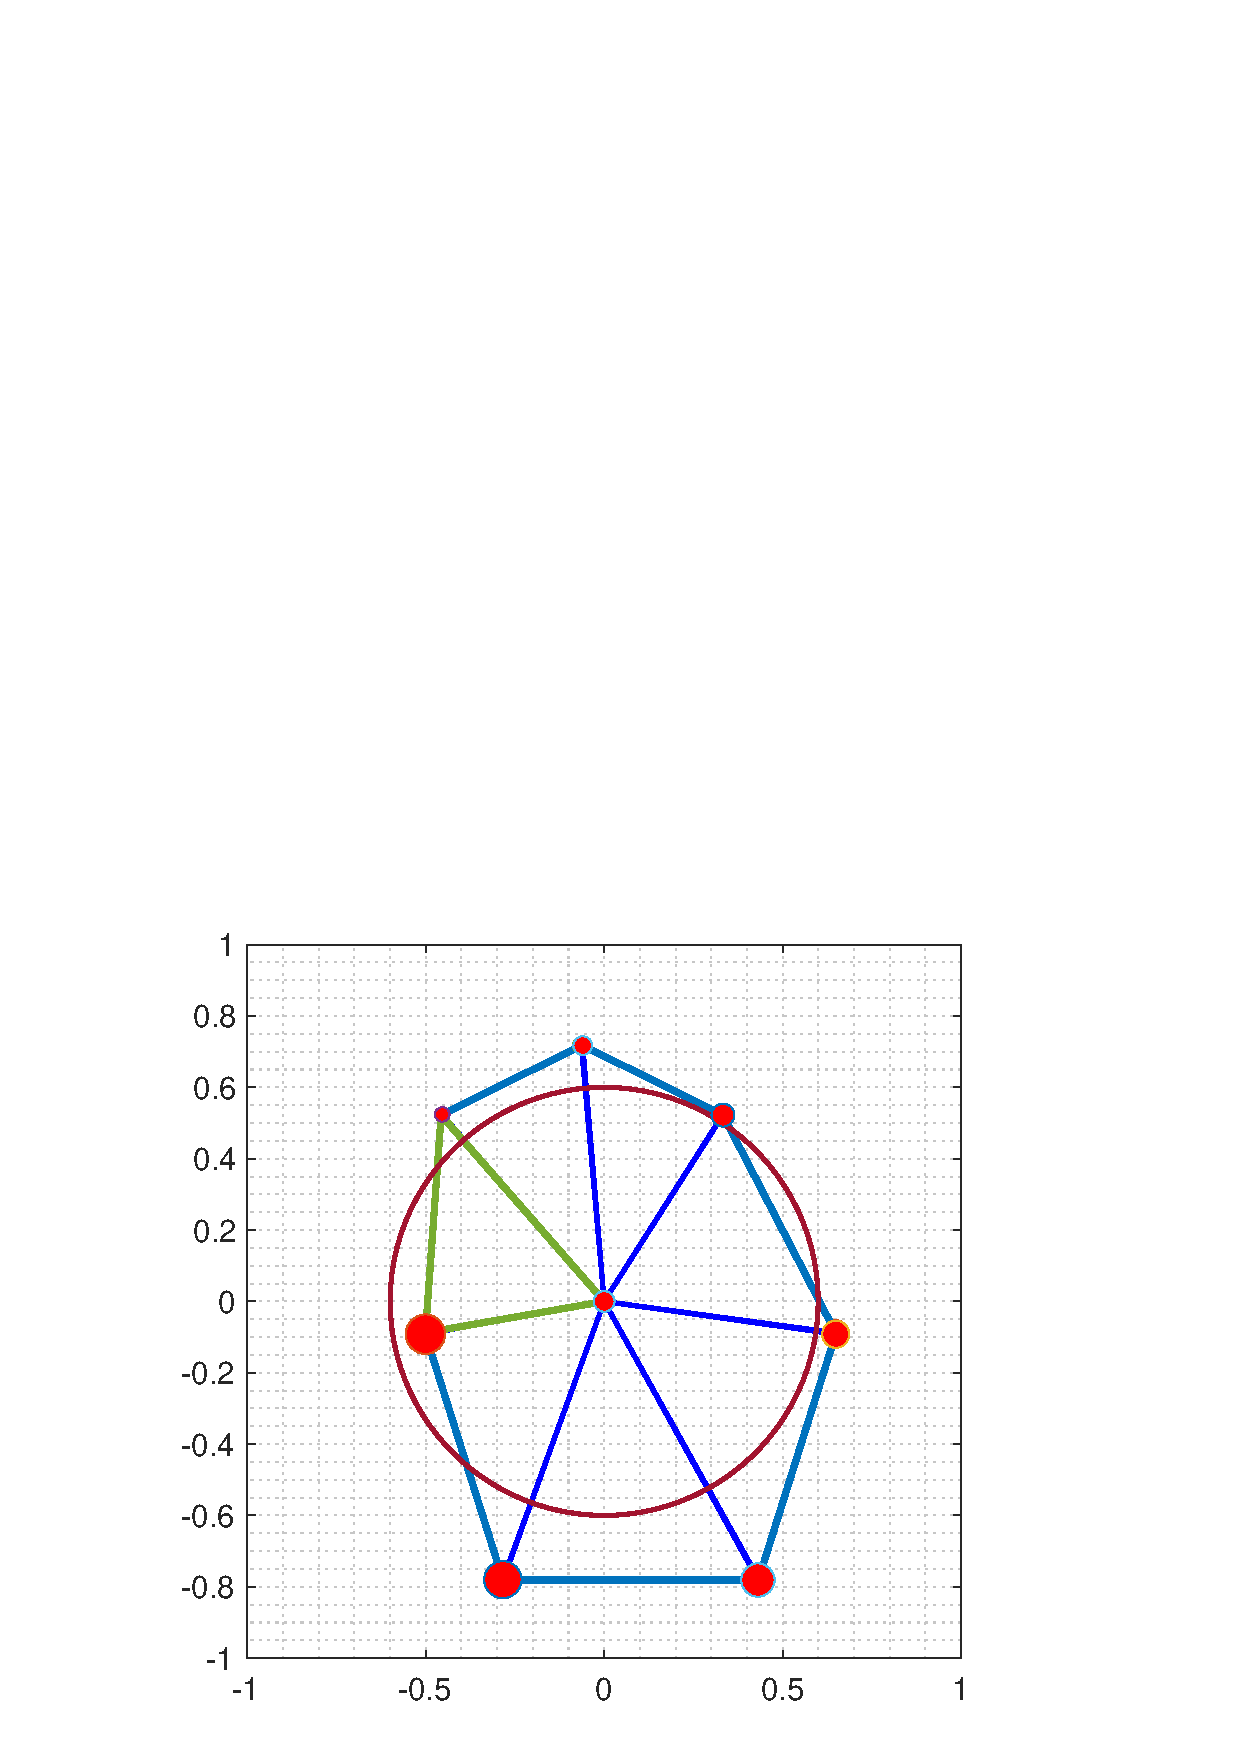
\includegraphics[width=0.8\textwidth]{Figures/1.png}
\caption{On the left: A square using the original timing pulley. On the right: The same 3D model square, but printed with the triangular pulley. We can not observe a modification in the y-axes, but in the x-axes be observe a relative reduction of 0.1.}
\end{figure}

\end{frame}



\setbeamercolor{background canvas}{bg=white!10}
\begin{frame}\frametitle{Circle test}

\begin{figure}[ht!]
\centering
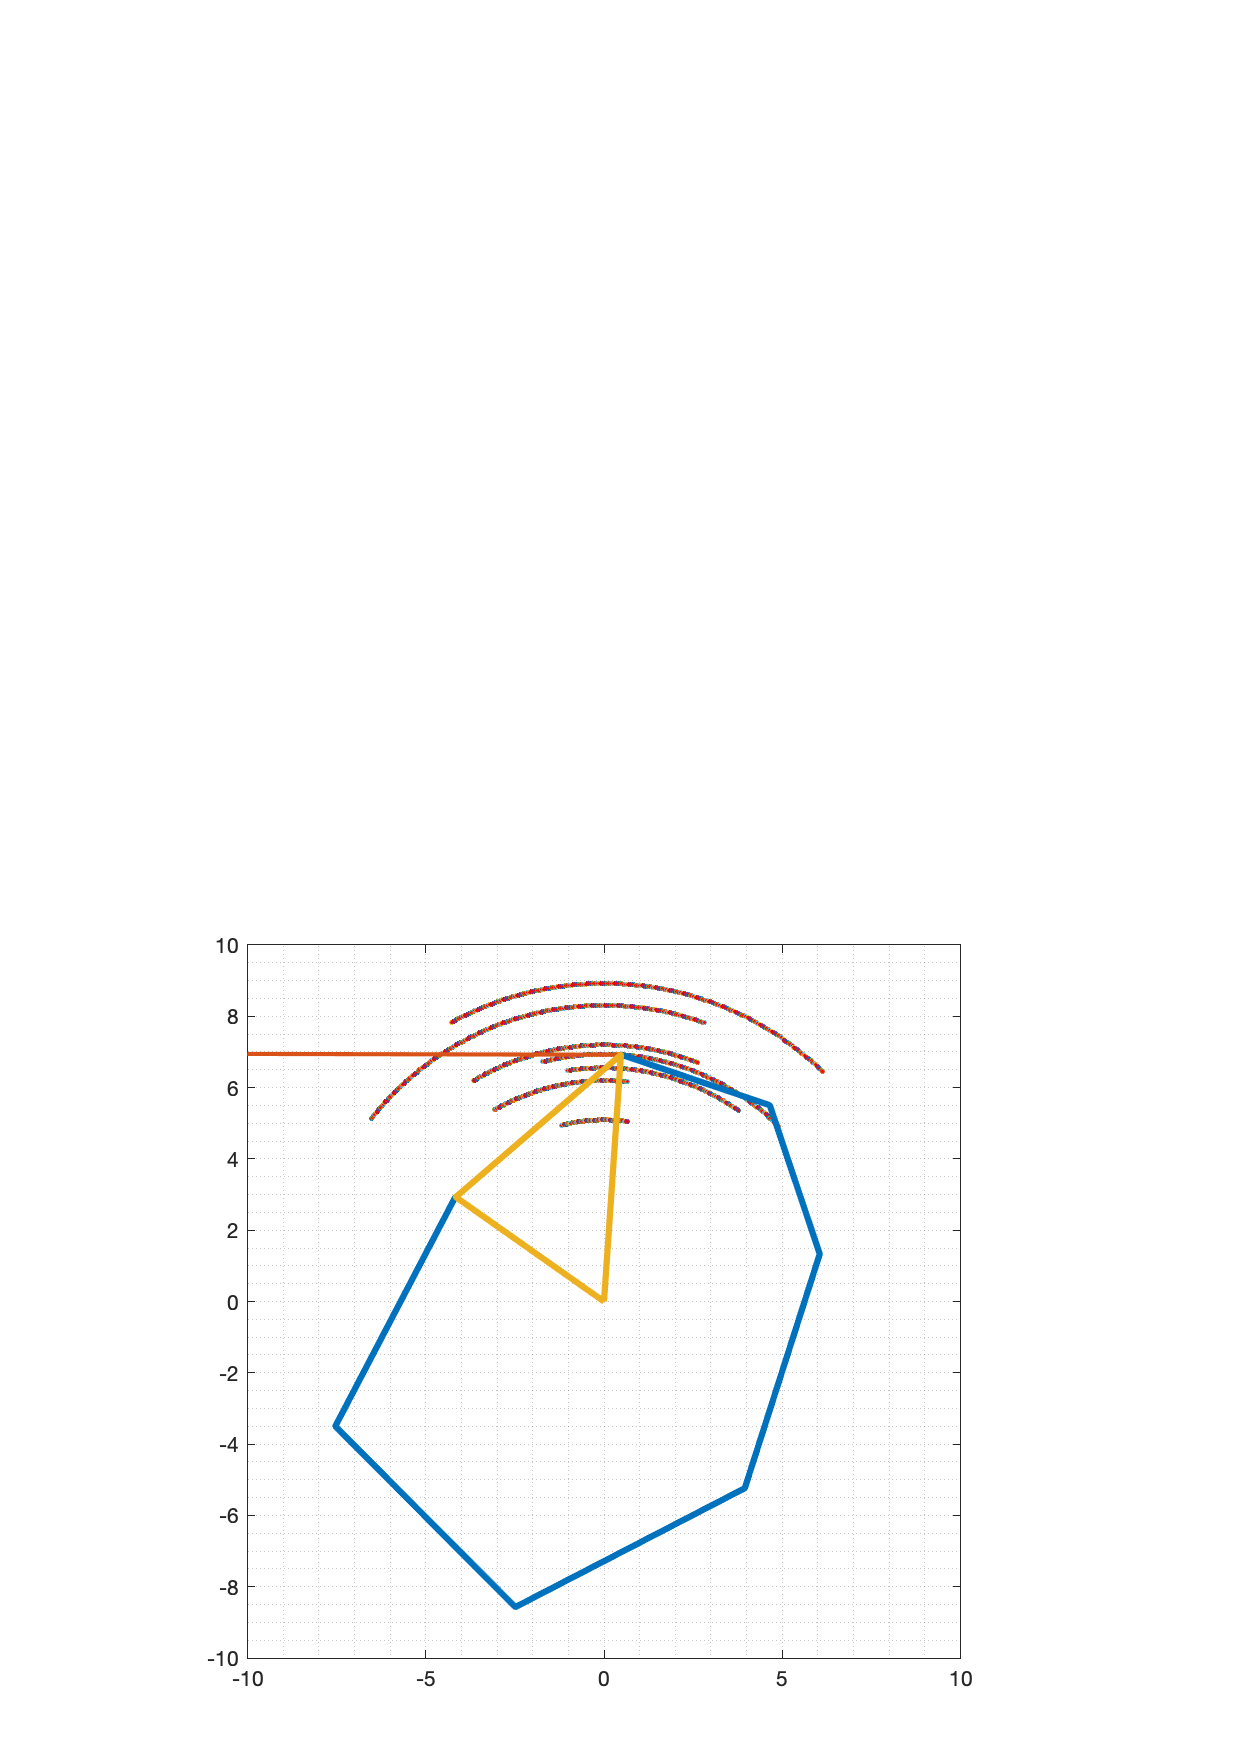
\includegraphics[width=0.8\textwidth]{Figures/2.png}
\caption{On the left: A circle using the original timing pulley. On the right: The same 3D model circle, but printed with the triangular pulley. We can not observe a modification in the y-axes, but in the x-axes be observe a relative reduction of 0.1.}
\end{figure}

\end{frame}



\setbeamercolor{background canvas}{bg=white!10}
\begin{frame}\frametitle{Correcting the 3D models}

When we consider this shrinking factor in the 3D models and stretch them before printing, we achieve the same shapes with the triangular pulley as they were printer with the original pulley (in grey printer with triangular pulley, while in yellow with original pulley).

\begin{columns}[c]

\column{.5\textwidth}
\begin{figure}[ht!]
\centering
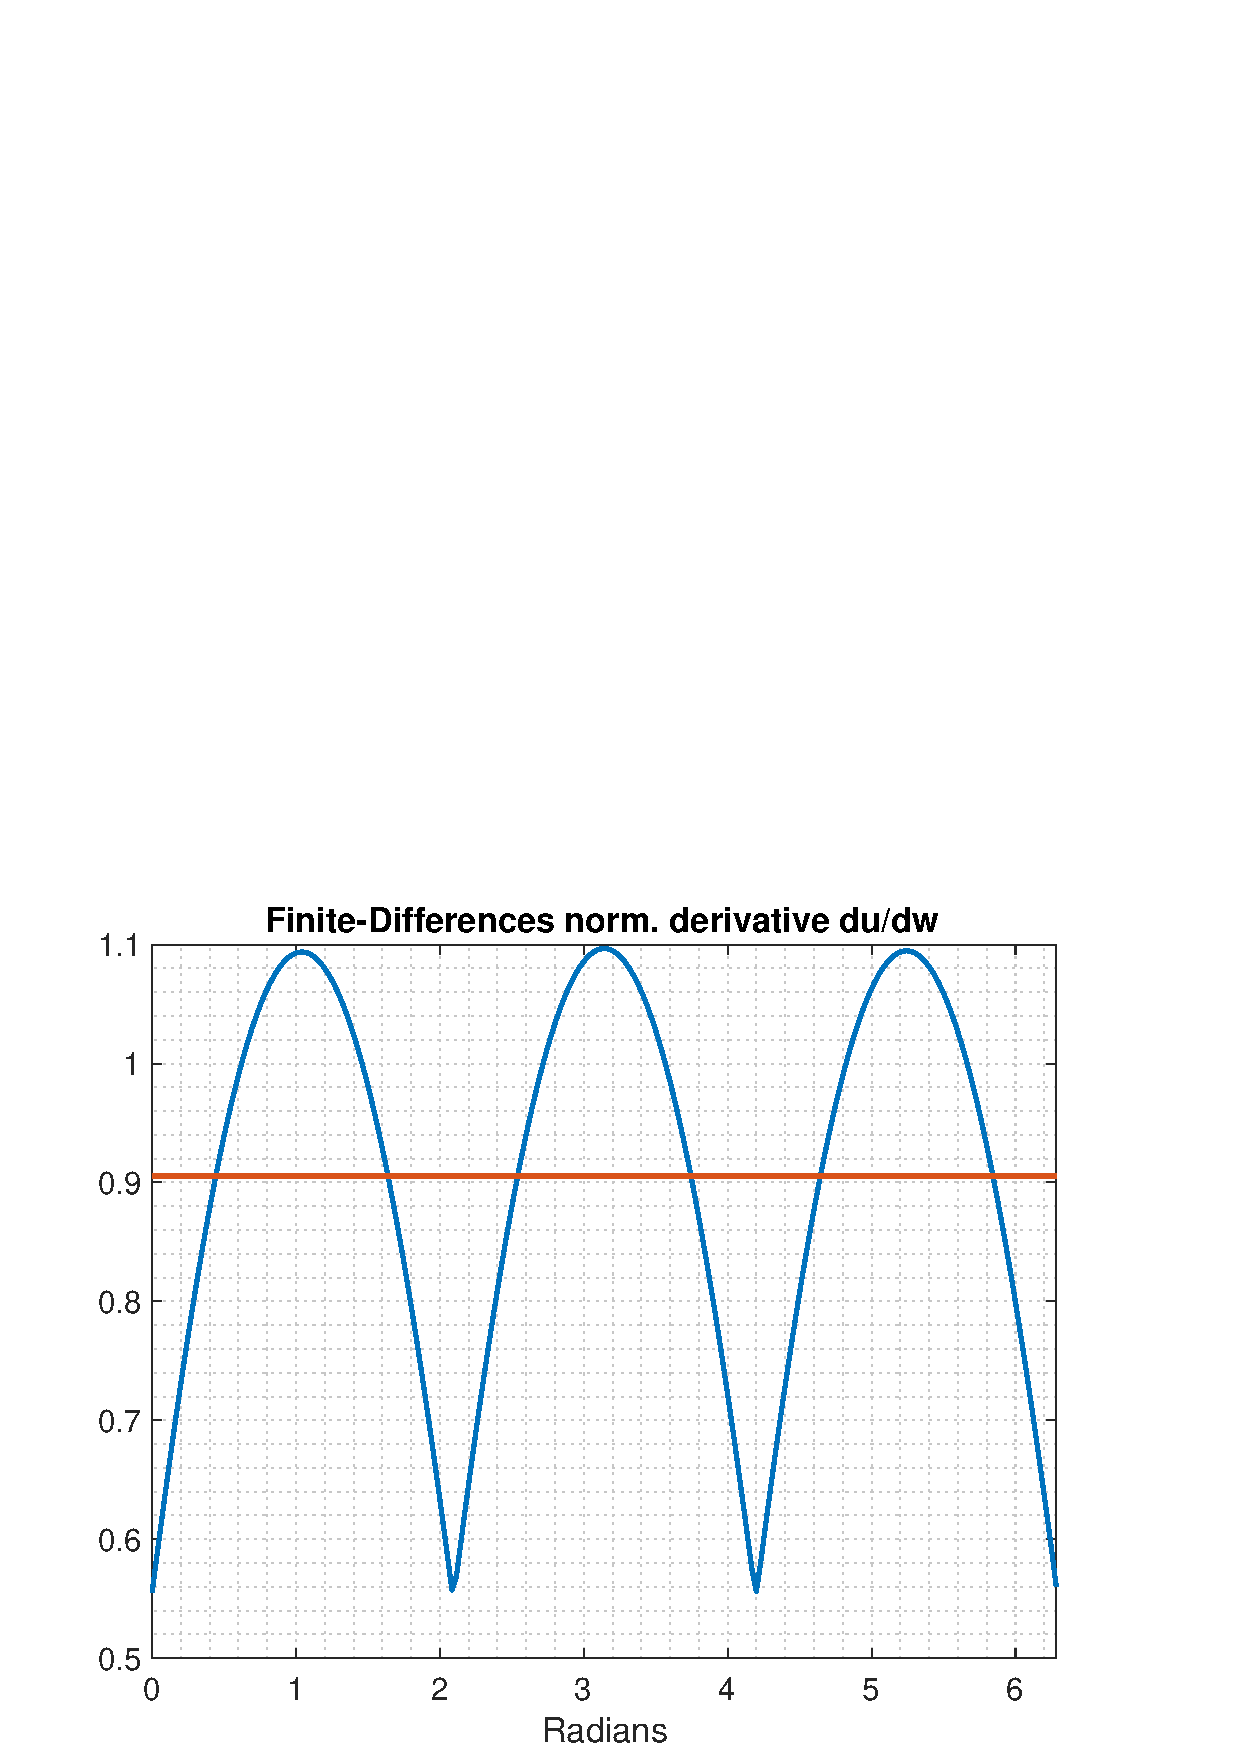
\includegraphics[width=0.8\textwidth]{Figures/3.png}
\end{figure}

\column{.5\textwidth}
\begin{figure}[ht!]
\centering
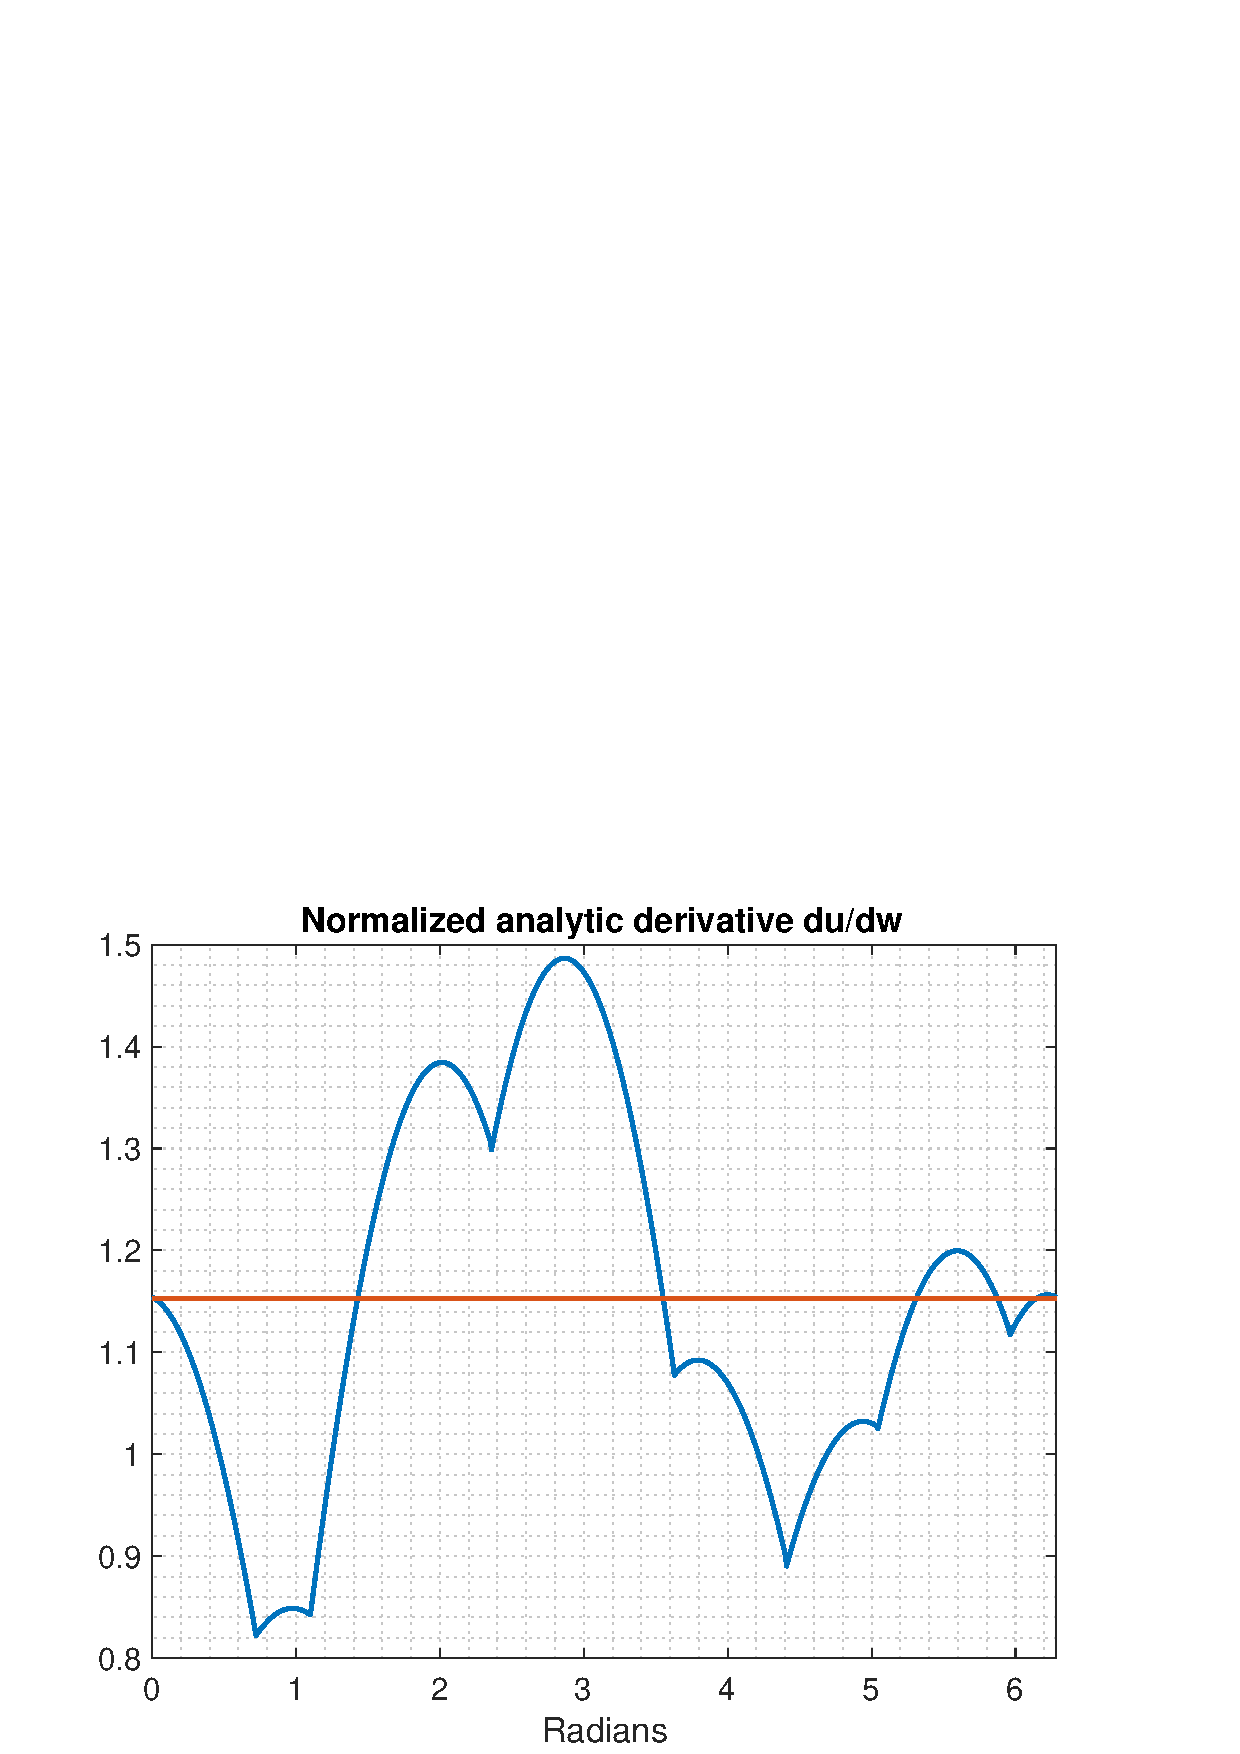
\includegraphics[width=0.8\textwidth]{Figures/4.png}
\end{figure}

\end{columns}

\end{frame}



\setbeamercolor{background canvas}{bg=white!10}
\begin{frame}\frametitle{Conclusions}

The triangular pulley shrinks the 3D models. We still need to do the calculations, but the triangular pulley makes the belt to advance less per rotation w.r.t. the original pulley.

\end{frame}



\setbeamercolor{background canvas}{bg=green!10}
\begin{frame}\frametitle{Extra: learning and self-awareness}

\begin{columns}[c]

\column{.45\textwidth}
\begin{figure}[ht!]
\centering
\includegraphics[width=0.8\textwidth]{Figures/5.png}
\end{figure}

\column{.45\textwidth}
That picture is from the game \textbf{Sims 2}. I thought we could make a robot learn to survive if we define some needs and let it find a way to satisfy them. However, I noticed this is way far from self-awareness.\\
\quad\\
I must admit that it is even scary the idea to develop a self-awareness entity.

\end{columns}

\end{frame}



\setbeamercolor{background canvas}{bg=green!10}
\begin{frame}\frametitle{Extra 2: printed gift!}

\begin{columns}[c]

\column{.45\textwidth}
\begin{figure}[ht!]
\centering
\includegraphics[width=0.8\textwidth]{Figures/20201213_153202.jpg}
\end{figure}

\column{.45\textwidth}
I have something for your Christmas tree! Also, I deleted the 3D model, so it is unique! You can use it next year in case we do not meet before Christmas!

\end{columns}

\end{frame}


%\setbeamercolor{background canvas}{bg=white!10}
%\begin{frame}\frametitle{Title}
%
%\begin{columns}[c]
%
%\column{.5\textwidth}
%
%\column{.5\textwidth}
%\begin{figure}[ht!]
%\centering
%\includegraphics[width=0.4\textwidth]{Figures/20190809_1.png}
%\end{figure}
%
%\end{columns}
%
%\end{frame}

\end{document}